%! TEX program = xelatex
\documentclass{cumcmthesis}
    %\documentclass[withoutpreface,bwprint]{cumcmthesis} %去掉封面与编号页

    \title{论文题目}
    \tihao{C}            % 题号
    \baominghao{4321}    % 报名号
    \schoolname{中山大学}
    \membera{陈昊蔚}
    \memberb{李可乐}
    \memberc{蔡佳陆}
    \supervisor{指导老师}
    \yearinput{2025}     % 年
    \monthinput{9}      % 月
    \dayinput{5}        % 日

    \begin{document}
        \maketitle
        \begin{abstract}
            摘要的具体内容。
            \keywords{Pearson检验\quad Spearman检验\quad  多元非线性回归分析\quad   粒子群算法\quad
            NIPT技术\quad 胎儿染色体异常\quad}
        \end{abstract}
        % \tableofcontents
        \section{问题重述}
        本节旨在提取题目的关键信息,全面概括关于NIPT时点选择与胎儿异常判定的背景,
        并进一步明确根据孕妇的BMI、孕周数、孕情等个体差异,推断出既能确保准确性、又能
        尽量降低治疗窗口期缩短的风险的最佳NIPT时点以及针对女胎异常的判定方法的现实要求,
        从而更加清晰地把握问题的核心要点。

        \subsection{问题背景}
        
        进入新时代,为了响应国家“晚婚晚育、少生优生”的号召,切实提高人口素质,
        许多家庭选择在较晚的年龄生育子女。然而,随着高龄产妇比例的增加,胎儿染色体异常的风险也随之上升。
        因此,如何在孕期早期准确筛查出胎儿染色体异常,成为了产前诊断领域亟需解决的重要问题。
        \par 
        NIPT(Non-Invasive Prenatal Test,无创产前检测)是一种产前检测技术,仅需对孕妇采集血样就可检测出其中的
        胎儿游离DNA片段,并分析胎儿染色体是否存在异常(例如唐氏综合征患者的21号染色体数量异常),从而在早期
        就可掌握胎儿的健康状况。NIPT技术可以有效筛查唐氏综合征、爱德华氏综合征和帕陶氏综合征这三大染色体异常疾病,
        准确率远超先前其他方法。此外,NIPT技术无需侵入性操作,避免了传统产前诊断方法可能带来的流产风险和对胎儿可能造成
        的伤害,因而被广泛应用于临床实践中。
        \par 我们本次研究的核心任务,便是基于一批孕妇的NIPT检测数据,
        构建有效的数学模型。我们希望能够借助数学模型分析胎儿Y染色体浓度和孕妇孕情的关系、不同BMI孕妇的最佳NIPT时点以及针对无Y染色体的女胎的异常判定
        方法等一系列问题。
        因此,如何利用现代数据分析与数学建模技术,排除或修正这些数据中潜在的干扰,
        准确地对上述问题完成模型建立与求解,成为了一个兼具医学意义与数据科学挑战的交叉学科课题。
        
        \subsection{基本问题}
        附件是某地区BMI偏高孕妇的NIPT检测数据,包含了孕妇的基本信息、孕情信息以及NIPT检测结果等内容。
        为了依据相关数据完成对更多孕妇的NIPT时点判断以及针对女胎的异常判定工作,现需要结合这些数据
        和已知条件,建立数学模型,分析以下问题:
        \par 
        \textbf{问题一}:依据男胎检测数据,分析胎儿Y染色体浓度与孕妇的孕周数和BMI等指标之间的相关特性,
        对有相关性的指标进行筛选,并建立数学模型,描述胎儿Y染色体浓度与孕妇孕周数和BMI等指标之间的关系。之后,再
        检验该模型的显著性。
        \par
        \textbf{问题二}:依据男胎检测数据,建立数学模型,对男胎孕妇的BMI进行分组,分析不同组别男胎孕妇的最佳NIPT时点,并
        分析检测误差对判断最佳NIPT时点的影响。
        \par
        \textbf{问题三}:依据男胎检测数据,综合考虑孕妇的身高、体重、年龄、生育次数等多种因素的影响,
        并结合检测误差以及胎儿Y染色体浓度达标比例,对孕妇的BMI进行再次分组,分析各组别孕妇的最佳NIPT时点,
        并分析检测误差对判断最佳NIPT时点的影响。
        \par
        \textbf{问题四}:依据女胎检测数据,建立数学模型,综合考虑X染色体和其他检测染色体的NIPT结果Z值、GC含量
        、读数段及相关比例、BMI等因素,分析女胎孕妇的21号、18号、13号染色体非整倍体结果,给出判断女胎是否异常的方法。
        \section{问题分析}
        \subsection{问题一分析}
        问题一要求我们依据男胎检测数据,分析胎儿Y染色体浓度与孕妇的孕周数和BMI等指标之间的相关特性。
        首先,我们需要对数据进行预处理,使得数据尽可能完整、合理。然后,我们可以使用统计分析方法,如Pearson检验和Spearman
        检验的相关系数计算和多元非线性回归分析,
        来探索胎儿Y染色体浓度与孕妇孕周数和BMI等指标之间的关系。通过建立数学模型,我们可以量化这些关系,并检验模型的显著性,以确保其可靠性。
        \par 具体步骤包括:
        \begin{itemize} 
            \item 数据预处理:清洗数据,处理缺失值和异常值。
            \item 相关性分析:计算胎儿Y染色体浓度与孕妇孕周数和BMI等指标的相关系数。
            \item 模型建立:选择合适的回归模型(如多项式回归等)来描述这些关系。
            \item 模型检验:使用合适的指标(t检验、RMSE、调整后$\text{R}^2$等)来评估模型的显著性和拟合优度。
        \end{itemize}
        \subsection{问题二分析}
        问题二指出,影响Y染色体浓度检测结果的主要因素是孕妇的BMI。基于此,我们需要对男胎孕妇的BMI进行区间划分,
        对于每个组别,分析其最佳NIPT时点。由于检测时间过晚可能会导致错过最佳治疗窗口期,
        因此为了满足题意中的“尽量降低治疗窗口期缩短的风险”,我们应当在确保检测的准确性,也就是Y染色体
        浓度大于等于4\%的前提下,选择尽可能早的NIPT时点。我们将各组别的最佳NIPT时点乘以该组别的权重,
        求和作为总的检测风险值,并以此作为优化目标,使用粒子群算法等优化方法来求解各组别的最佳NIPT时点。
        \par
        

        
        \section{模型假设}
        结合题意和上述对问题的分析,为了合理简化模型的建立与求解过程,我们提出了以下假设:
        \begin{itemize}
            \item \textbf{假设1}:数据中的测量误差是随机分布的,不会系统性地偏向某一方向。
            \item \textbf{假设2}:孕妇的身体状况和生活习惯等非NIPT检测指标在研究期间保持相对稳定,不会对胎儿Y染色体浓度产生显著影响。
            \item \textbf{假设3}:不同孕妇之间的个体差异可以通过统计方法进行控制和调整。
            \item \textbf{假设4}:胎儿Y染色体浓度与孕妇的孕周数和BMI等指标之间的关系可以通过多元非线性回归模型进行描述。
            \item \textbf{假设5}:在问题二和问题三中,孕妇的BMI分组是合理且具有代表性的。考虑到各组别中BMI的分布不一定足够均匀,
            假定每个组别的BMI中位数对应的最佳NIPT时点能够代表该组别的最佳NIPT时点。
            \item \textbf{假设6}:孕妇的潜在风险仅取决于NIPT时点的选择,而不受其他外部因素的影响。
        \end{itemize}
        \section{符号说明}
        \begin{center}
            \begin{tabular}{cc}
                \hline
                \makebox[0.3\textwidth][c]{\textbf{概念/符号}}	&  \makebox[0.4\textwidth][c]{\textbf{意义}} \\ \hline
                
                BMI     &  身体质量指数,BMI = 体重(kg)/$\text{身高}^2\text{(m}^2 \text{)}$ \\ 
                Z值  &   数据经过Z-Score标准化后得到的数值  \\ 
                $Y$ & 胎儿Y染色体浓度 \\
                $X_1$ & 孕周数 \\
                $X_2$ & 孕妇BMI \\
                $t_i$ & 第$i$组别的最佳NIPT时点 \\
                $w_i$ & 第$i$组别的权重 \\
                 $f(t_1,t_2,t_3,t_4,t_5)$ & 总的检测风险值 \\
                 $N$ & 总的孕妇人数 \\
                 $n_i$ & 第$i$组别的孕妇人数 \\
                \hline
            \end{tabular}
        \end{center}
        \section{模型的建立与求解}

        \subsection{问题一的模型建立与求解}
            \subsubsection{数据预处理}
                在进行建模之前,我们应当对附件原始数据进行合理的预处理,包括以下几个方面:
                \par
                \textbf{缺失值处理}:对于缺失的数据,采用均值填补、插值法或删除含有缺失值的样本等方法进行处理。
                \begin{figure}[htbp]
                \centering
                \includegraphics[width=12cm]{D:/Code/Competitions/CUMCM2025/pic/BMI箱线图.pdf}
                \caption{男胎孕妇BMI箱线图}
                \label{fi1}
                \end{figure}
                \par
                \textbf{异常值检测}:使用箱线图识别BMI等变量中的异常值,并根据具体情况决定是否剔除或修正这些异常值。
                使用Python绘制BMI的箱线图,发现在上须线以上有大量异常点,在下须线以下存在一个异常点,如图1所示。
                
                经过使用身高、体重的原始数据重新计算BMI,我们发现异常值与重新计算值的相对误差不超过
                $1\textperthousand$。然而,由于题意中描述的数据人群主要是BMI较大的孕妇,因此BMI为25以下的,我们
                将其视为离群值,予以舍弃。对于上述在上须线以上的异常值,我们则选择保留。
                \par
                此外,对于Y染色体浓度超过$20\%$的异常值,显然已经不符合生物学常识,可能是检测错误,因此我们选择剔除这些异常值。
                \par
                \textbf{纵向数据整理}:对于“一次抽血多次检验”的数据,取其中位数作为该孕妇的最终检测结果,以减少偶然误差的影响。
                

            \subsubsection{相关性检验}
                为了分析胎儿Y染色体浓度与孕妇的孕周数和BMI等指标之间的相关特性,我们首先计算这些变量之间的相关系数。
                \par
                由于BMI和孕周数均为连续变量,我们可以使用Pearson相关系数来衡量它们与Y染色体浓度之间的线性关系。同时考虑到
                该关系也有可能是非线性的,因此我们也计算了Spearman秩相关系数,以便交互验证。计算得到的两种相关系数热力图如图2所示。
                \begin{figure}[htbp]
                \centering
                \includegraphics[width=16.5cm]{D:/Code/Competitions/CUMCM2025/pic/Pearson与Spearman相关系数热力图.pdf}
                \caption{Pearson与Spearman相关系数热力图}
                \label{fi2}
                \end{figure}
                \begin{figure}[htbp]
                \centering
                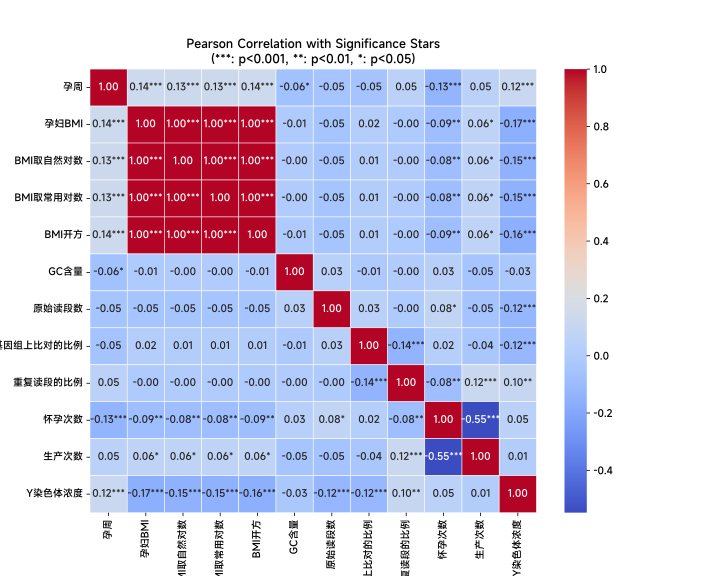
\includegraphics[width=12cm]{D:/Code/Competitions/CUMCM2025/pic/Pearson相关系数.pdf}
                \caption{Pearson相关系数和P值热力图}
                \label{fi3}
                \end{figure}
                \par
                由图3可见,与Y染色体浓度的相关性检验满足P值法的因素有:孕周、BMI、原始读段数、在参考基因组上比对的比例、
                重复读段的比例等。然而,显然“原始读段数”“在参考基因组上比对的比例”和“重复读段的比例”仅仅是判断NIPT检测过程中
                样本量是否足够大、是否有重复测量的技术指标,并不具备生物学意义,因此我们将其排除在影响Y染色体浓度的因素之外。
                对于剩下的因素,可以发现Y染色体浓度与孕周数和孕妇BMI的P值均小于0.001,表明两者与Y染色体浓度之间均存在显著的相关性。
                同时又可以发现Y染色体浓度与孕周数的Pearson相关系数和Spearman相关系数均为接近0的正数,表明两者之间存在正向的关系,
                但是线性相关性很弱;同理,Y染色体浓度与孕妇BMI的Pearson相关系数和Spearman相关系数均为接近0的负数,表明两者之间存在负向关系,
                但是线性相关性也很弱。
                \par
                综合上述分析结果,我们决定在后续模型中同时考虑孕周数和BMI对Y染色体浓度的影响,并重点考虑两者之间可能存在的非线性关系。
            \subsubsection{回归模型建立与显著性的检验}
                由于Y染色体浓度与孕周数和BMI之间的相关性较弱,我们决定采用多元线性回归模型以及多元非线性回归模型来
                先后尝试描述它们之间的关系,后者主要包括包含交互项的二阶多项式回归模型、包含交互项的三
                阶多项式回归模型和双对数模型。
                其函数模型如表1所示。
                其中,$Y$表示Y染色体浓度,$X_1$表示孕周数,$X_2$表示BMI,$\beta_i(i=1,2,\dots)$和$d$均为待定系数。
            \begin{table}[htbp]
            \centering
            \begin{tabular}{cc}
            \hline
            \makebox[0.3\textwidth][c]{\textbf{模型名称}} & \makebox[0.4\textwidth][c]{\textbf{定义公式}} \\
            \hline
            %多元线性回归模型 & 
            %$Y=\beta_1 X_1+\beta_2 X_2+d$ \\
            包含交互项的二阶多项式回归模型 & 
            $Y=\beta_1 X_1^2+\beta_2 X_2^2+\beta_3 X_1X_2+\beta_4 X_1+\beta_5 X_2+d$
            \\
            包含交互项的三阶多项式回归模型 & 
            $ \begin{aligned}
                Y&=\beta_1 X_1^3+\beta_2 X_2^3+\beta_3 X_1^2X_2+\beta_4 X_1X_2^2+\beta_5 X_1^2\\
                                        &+\beta_5 X_1^2+\beta_6 X_2^2+\beta_7 X_1 X_2+\beta_8 X_1+\beta_9 X_2+d
                \end{aligned} $
            \\
            双对数模型 & 
            $ \ln Y=\beta_1 + \beta_2 \ln X_1 +\beta_3 \ln X_2$ \\
            \hline
            \end{tabular}
            \caption{问题一的回归模型建立}
            \end{table}
            
            \par
            经过计算,我们得到了各个模型的待定系数,并使用调整后的$\text{R}^2$、
            RMSE和AIC等指标对各个模型的拟合优度进行了评估,同时为了检验该模型的显著性,
            还做了对模型整体的F检验,结果如表2所示。
             \begin{table}[htbp]
            \centering
            \begin{tabular}{cccccc}
            \hline
            {\textbf{模型名称}}  & {RMSE} &{AIC}&{BIC}&{$\text{调整后R}^2$}&{F检验的P值} \\
            \hline
            %多元线性回归模型 &\\
            二阶多项式回归模型 & 0.0307 &-7050.1141 &-7020.5841 &0.0650 &1.0000
            \\
            三阶多项式回归模型 & 0.0303&-7070.2017&-7020.9851&0.0906 &1.0000
            
            \\
            双对数模型 & 0.0319&-6978.2983&-6963.5333&~&0
            \\
            \hline
            \end{tabular}
            \caption{问题一的回归模型指标比较}
            \end{table}
            \par
            由表2可见,尽管包含交互项的三阶多项式回归模型在各项指标上均优于其他模型,但由于其F检验
            的P值过大,因而我们选择相对更加稳健的双对数模型作为最终的回归模型。
            经过计算,我们得到了该模型的待定系数为$\beta_1=\text{0.8528}$,$\beta_2=\text{0.2305}$,$\beta_3=\text{-0.9045}$。
            所以问题一的回归模型为
            \begin{equation}
                \ln Y=0.9004 + 0.2299 \ln X_1 -0.9195 \ln X_2
            \end{equation}
            该函数的拟合效果如图4所示。
            \begin{figure}[htbp]
            \centering
            \includegraphics[width=16cm]{D:/Code/Competitions/CUMCM2025/pic/对比图.pdf}
            \caption{问题一的回归模型拟合效果}
            \label{fi4}
            \end{figure}
        \subsection{问题二的模型建立与求解}
            \subsubsection{确立优化模型}
            参考题干中提到的分组举例,我们先假定可以将BMI划分为5组。由于在达到Y染色体浓度大于等于4\%,也即NIPT检测准确率有所保障的前提下,
            孕妇做NIPT检测的时间越早则对孕妇和胎儿的后续检测和治疗风险越小,因此我们利用“时间早”和“风险小”的一致性,将风险函数定义为
            各组别的最佳NIPT时点乘以该组别的权重之和,也即
            \begin{equation}
                f(t_1,t_2,t_3,t_4,t_5)=\sum_{i=1}^5 w_i \cdot t_i
            \end{equation}
            其中,$w_i=\displaystyle\frac{n_i}{N}$。同时,为了确保NIPT检测的准确性,我们还需要添加约束条件如下:
            \begin{itemize}
                \item $t_i \geq 9$,即NIPT检测时点不早于孕9周(对于绝大多数数据样本,9周以前的Y染色体浓度均小于4\%);
                \item $t_i \leq 24$,即NIPT检测时点不晚于孕28周(由题意知,28周以后发现异常风险极高);
                \item $n_i \geq 20$,即每个组别的孕妇人数不少于20人。
            \end{itemize}
            \par
            综上所述,我们可以将问题二的优化模型表述为:
           \begin{equation}
            \min f(t_1,t_2,t_3,t_4,t_5)=\sum_{i=1}^5 w_i \cdot t_i
            \\ 
           \end{equation}
           \[\text{s.t.}\begin{cases}9\leq t_i\leq 24 & ,i=1,2,\dots,5\\n_i\geq 20&,i=1,2,\dots,5\end{cases}\]
           \par
            \subsubsection{粒子群算法求解BMI分组与各组别最佳NIPT时点}
            得到了上述目标函数和约束条件后,我们便可以使用粒子群算法来求解各组别的最佳NIPT时点。
        \subsection{问题三的模型建立与求解}
        \subsection{问题四的模型建立与求解}
        \section{总结}
        \begin{thebibliography}{9}%宽度9
            \bibitem{bib:one} ....
        \end{thebibliography}
        \begin{appendices}
            附录的内容。
        \end{appendices}
\end{document}